\documentclass[UTF8,a4paper,11pt]{ctexart}
\usepackage[margin=22mm,headheight=14pt,footskip=13mm]{geometry}
\usepackage{fontspec}
\usepackage{tabularx,booktabs,array,graphicx,xcolor,tikz,enumitem,hyperref,fancyhdr,microtype}
\usetikzlibrary{arrows.meta,positioning,fit,calc}
\setCJKmainfont{Noto Sans CJK SC}
\setCJKsansfont{Noto Sans CJK SC}
\setmainfont{TeX Gyre Heros}
\setsansfont{TeX Gyre Heros}
\definecolor{navy}{HTML}{173451}
\definecolor{blue}{HTML}{14577D}
\definecolor{pale}{HTML}{EAF2F7}
\hypersetup{colorlinks=true,urlcolor=blue,linkcolor=blue,pdftitle={星火NPU设计报告},pdfauthor={李建昊}}
\pagestyle{fancy}\fancyhf{}\fancyhead[L]{\small 星火 NPU｜设计报告}\fancyhead[R]{\small 流片支持申请}\fancyfoot[C]{\small\thepage}
\renewcommand{\headrulewidth}{0.3pt}
\setlength{\parindent}{2em}\setlength{\parskip}{0.25em}
\setlist[enumerate]{leftmargin=2em,itemsep=0.35em,topsep=0.35em}
\graphicspath{{output/pdf/}{./}}
\ctexset{section={format=\large\bfseries\color{blue},beforeskip=1.15em,afterskip=0.45em}}
\newcommand{\metric}[1]{\textbf{#1}}
\begin{document}
\begin{center}
{\LARGE\bfseries\color{navy}“星火”NPU 设计报告}\par\vspace{0.35em}
{\small 面向 MPSoC-Digital 平台的数字 Tile｜ICS55 工艺｜150\,MHz 目标时钟}\par
{\small 作者：李建昊}\par
\end{center}
\vspace{0.3em}
\noindent\colorbox{pale}{\parbox{\dimexpr\linewidth-2\fboxsep\relax}{\small 本报告对应同时提交的 \texttt{xinghuo-npu-tile.v}（门级网表）与 \texttt{xinghuo-npu-tile.def}（布局文件），两者顶层均为 \texttt{Tile}。开源项目：\href{https://github.com/Briarcresy/XingHuo-NPU}{github.com/Briarcresy/XingHuo-NPU}。}}

\section{功能概述}
“星火”NPU 是一个面向小规模神经网络推理的教学型加速器。计算核心采用 $2\times2$ 权重固定（Weight Stationary）脉动阵列，包含四个 MAC（乘加）处理单元。数据路径完成有符号 INT8 乘法、INT32 累加及偏置相加，再经算术右移、INT8 饱和和 ReLU 得到输出。权重留在处理单元中，激活值与部分和沿阵列传播，避免为每次乘加重复装载权重。

Tile 控制器通过平台提供的 $256\times8$ Shared RAM（共享存储器）读取输入和参数，依次运行两层 $2\times2$ 网络；第一层实际计算结果作为第二层输入，最终写回隐藏层、输出、分类及状态。设计支持两种操作：拨码和按钮执行固定 XOR 演示；外部主机经 \texttt{customIn/customOut} 握手写入可编程权重、偏置与移位参数并启动计算。

\begin{figure}[htbp]\centering
\begin{tikzpicture}[>=Latex, font=\small, node distance=9mm,
 block/.style={draw=blue,rounded corners=2pt,fill=pale,align=center,minimum height=12mm,minimum width=27mm,inner sep=3pt},
 ext/.style={draw=gray!70,dashed,rounded corners=2pt,align=center,minimum height=12mm,minimum width=24mm,inner sep=3pt},
 flow/.style={->,thick,draw=navy}]
 \node[ext] (input) {按钮/拨码\\外部主机};
 \node[block,right=12mm of input] (front) {同步、去抖\\命令/模式控制};
 \node[block,right=12mm of front] (seq) {两层网络\\调度控制器};
 \node[block,right=12mm of seq] (core) {NPU Core\\$2\times2$ MAC 阵列 + VPU};
 \node[ext,below=11mm of seq] (ram) {SoC Shared RAM\\$256\times8$，Tile 外部};
 \node[ext,below=11mm of core] (out) {LED/七段显示\\主机状态与结果};
 \draw[flow] (input)--(front);\draw[flow] (front)--(seq);\draw[flow] (seq)--(core);
 \draw[flow] (core.south)--(out.north);
 \draw[flow] (seq.south)--node[left,font=\scriptsize]{地址/写数据}(ram.north);
 \draw[flow] ([xshift=4mm]ram.north)--node[right,font=\scriptsize]{读数据}([xshift=4mm]seq.south);
\end{tikzpicture}
\caption{Tile 功能架构示意。依据项目已有的 Tile 架构图简化重绘；共享 RAM 属于 SoC，图中模块分组不代表额外 RTL 层级。}
\end{figure}

\section{设计指标}
\begin{table}[htbp]\centering\small
\begin{tabularx}{\linewidth}{@{}p{0.24\linewidth}X@{}}\toprule
项目 & 设计指标与实现边界\\\midrule
计算规模 & $2\times2$ 阵列、4 个 MAC；硬件顺序执行两层 $2\times2$ 网络。\\
数值格式 & 有符号 INT8 输入/权重，INT32 累加/偏置，INT8 输出；算术右移量 0--31，并进行饱和与 ReLU。\\
工作时钟 & 目标 150\,MHz（周期约 6.67\,ns）；最终工作范围以整片集成及硅后测试为准。\\
系统接口 & MPSoC-Digital 固定 Tile 接口；8 位 LED/按钮/拨码、七段显示、16 位 \texttt{customIn/customOut} 与 $256\times8$ 共享 RAM 接口。\\
功能验证 & Python Golden Model（参考模型）、1016 组 Core 向量、160 组两层网络、协议和复位边界、官方 Unit/Harness、零延迟门级仿真。\\\bottomrule
\end{tabularx}
\end{table}

\clearpage
\section{综合与 ECOS Studio 物理实现}
数据来自随附网表和 DEF 对应的 ICS55、150\,MHz 后端运行，统计范围为\textbf{完整 Tile 数字逻辑}，包含计算核心、两层网络控制、接口及显示逻辑。综合使用 Yosys，后端流程使用 ECOS Studio；面积单位为 $\mu\mathrm{m}^2$。
\begin{table}[htbp]\centering\small
\begin{tabularx}{\linewidth}{@{}Xr@{}}\toprule
指标 & 结果\\\midrule
综合后标准单元数 & \metric{7,773 个}\\
综合标准单元面积 & \metric{16,672.88 $\mu\mathrm{m}^2$}\\
ECOS Studio Core（放置区域）面积 / 利用率 & \metric{55,790.28 $\mu\mathrm{m}^2$ / 30\%}\\
ECOS Studio Die（本 Tile 边界）面积 / 利用率 & \metric{57,695.88 $\mu\mathrm{m}^2$ / 29\%}\\
DEF \texttt{DIEAREA} 尺寸 & 239.8 $\times$ 240.6\,$\mu\mathrm{m}$\\
13 角 STA 最差 Setup / Hold 裕量 & +0.122 / +0.069\,ns\\
该后端流程的 DRC / LVS 违例数 & 0 / 0\\\bottomrule
\end{tabularx}
\end{table}

其中 30\% 是布局核心区的放置利用率，不能解释为整片 MPSoC 的面积占比。共享 RAM 由平台提供，不在本 Tile 内重复实例化。综合单元数是 Yosys 映射后的逻辑单元数；布线及填充后新增的物理实例不计入该数。13 角 STA 在此 Tile 的后端约束下建立和保持裕量均为正，DRC/LVS 检查为零违例；整片封装与平台集成仍须单独确认。

\section{回片后测试方法与预期效果}
\begin{enumerate}
\item \textbf{上电、复位与可访问性：}按平台规定连接电源、时钟和复位，确认 Tile 端口到封装/载板或平台固件的访问路径。复位至少覆盖三个有效时钟沿；检查状态、显示、RAM 写使能和主机请求应答。预期复位期间无意外 RAM 写入，请求握手正常。
\item \textbf{固定 XOR 冒烟测试：}依次设置 \texttt{DIP[1:0]} 为 \texttt{00/01/10/11}，输入稳定后按 \texttt{BTN7} 启动，等待完成并读取 LED 或 \texttt{customOut[13]}。预期分类依次为 \textbf{0、1、1、0}，四次运行均完成且无错误状态。
\item \textbf{可编程网络功能测试：}主机逐字节写入输入、两层权重/偏置/移位；启动后轮询 busy/done。读取 RAM \texttt{0x20--0x23} 的隐藏层、\texttt{0x40--0x43} 的输出，以及 \texttt{0x44--0x46} 的分类/状态/错误码，与 Python 参考模型逐字节比对。覆盖正负数、量化饱和、连续任务、忙时请求和复位恢复；预期数值一致且无丢失、重复事务。
\item \textbf{工作裕量测试：}在平台允许的电压、温度和时钟范围内重复上述向量，记录错误率、最高可靠频率及失效边界。预期在最终规定的工作条件内稳定运行；具体裕量由实测给出。
\end{enumerate}

\section{其他说明}
本设计强调小面积、可观察、可验证的两层 $2\times2$ 网络演示，参数可编程，但不提供通用神经网络指令集或大容量片上存储。上板测试需要平台确认时钟、复位、共享 RAM 读写时序以及外部引脚映射。现有功能验证和本 Tile 的后端检查不代替整片集成签核、Scan/ATPG（制造缺陷测试）或硅后性能评估。

\clearpage
\section{版图展示}
图\ref{fig:layout}为与随附网表、DEF 对应的 ECOS Studio 布局布线可视化。图示范围为本 Tile 的 $239.8\times240.6\,\mu\mathrm{m}$ 边界；Core 放置利用率为 30\%。彩色线条呈现单元与布线分布，精确的几何与连接信息以随附 DEF 为准。
\begin{figure}[htbp]\centering
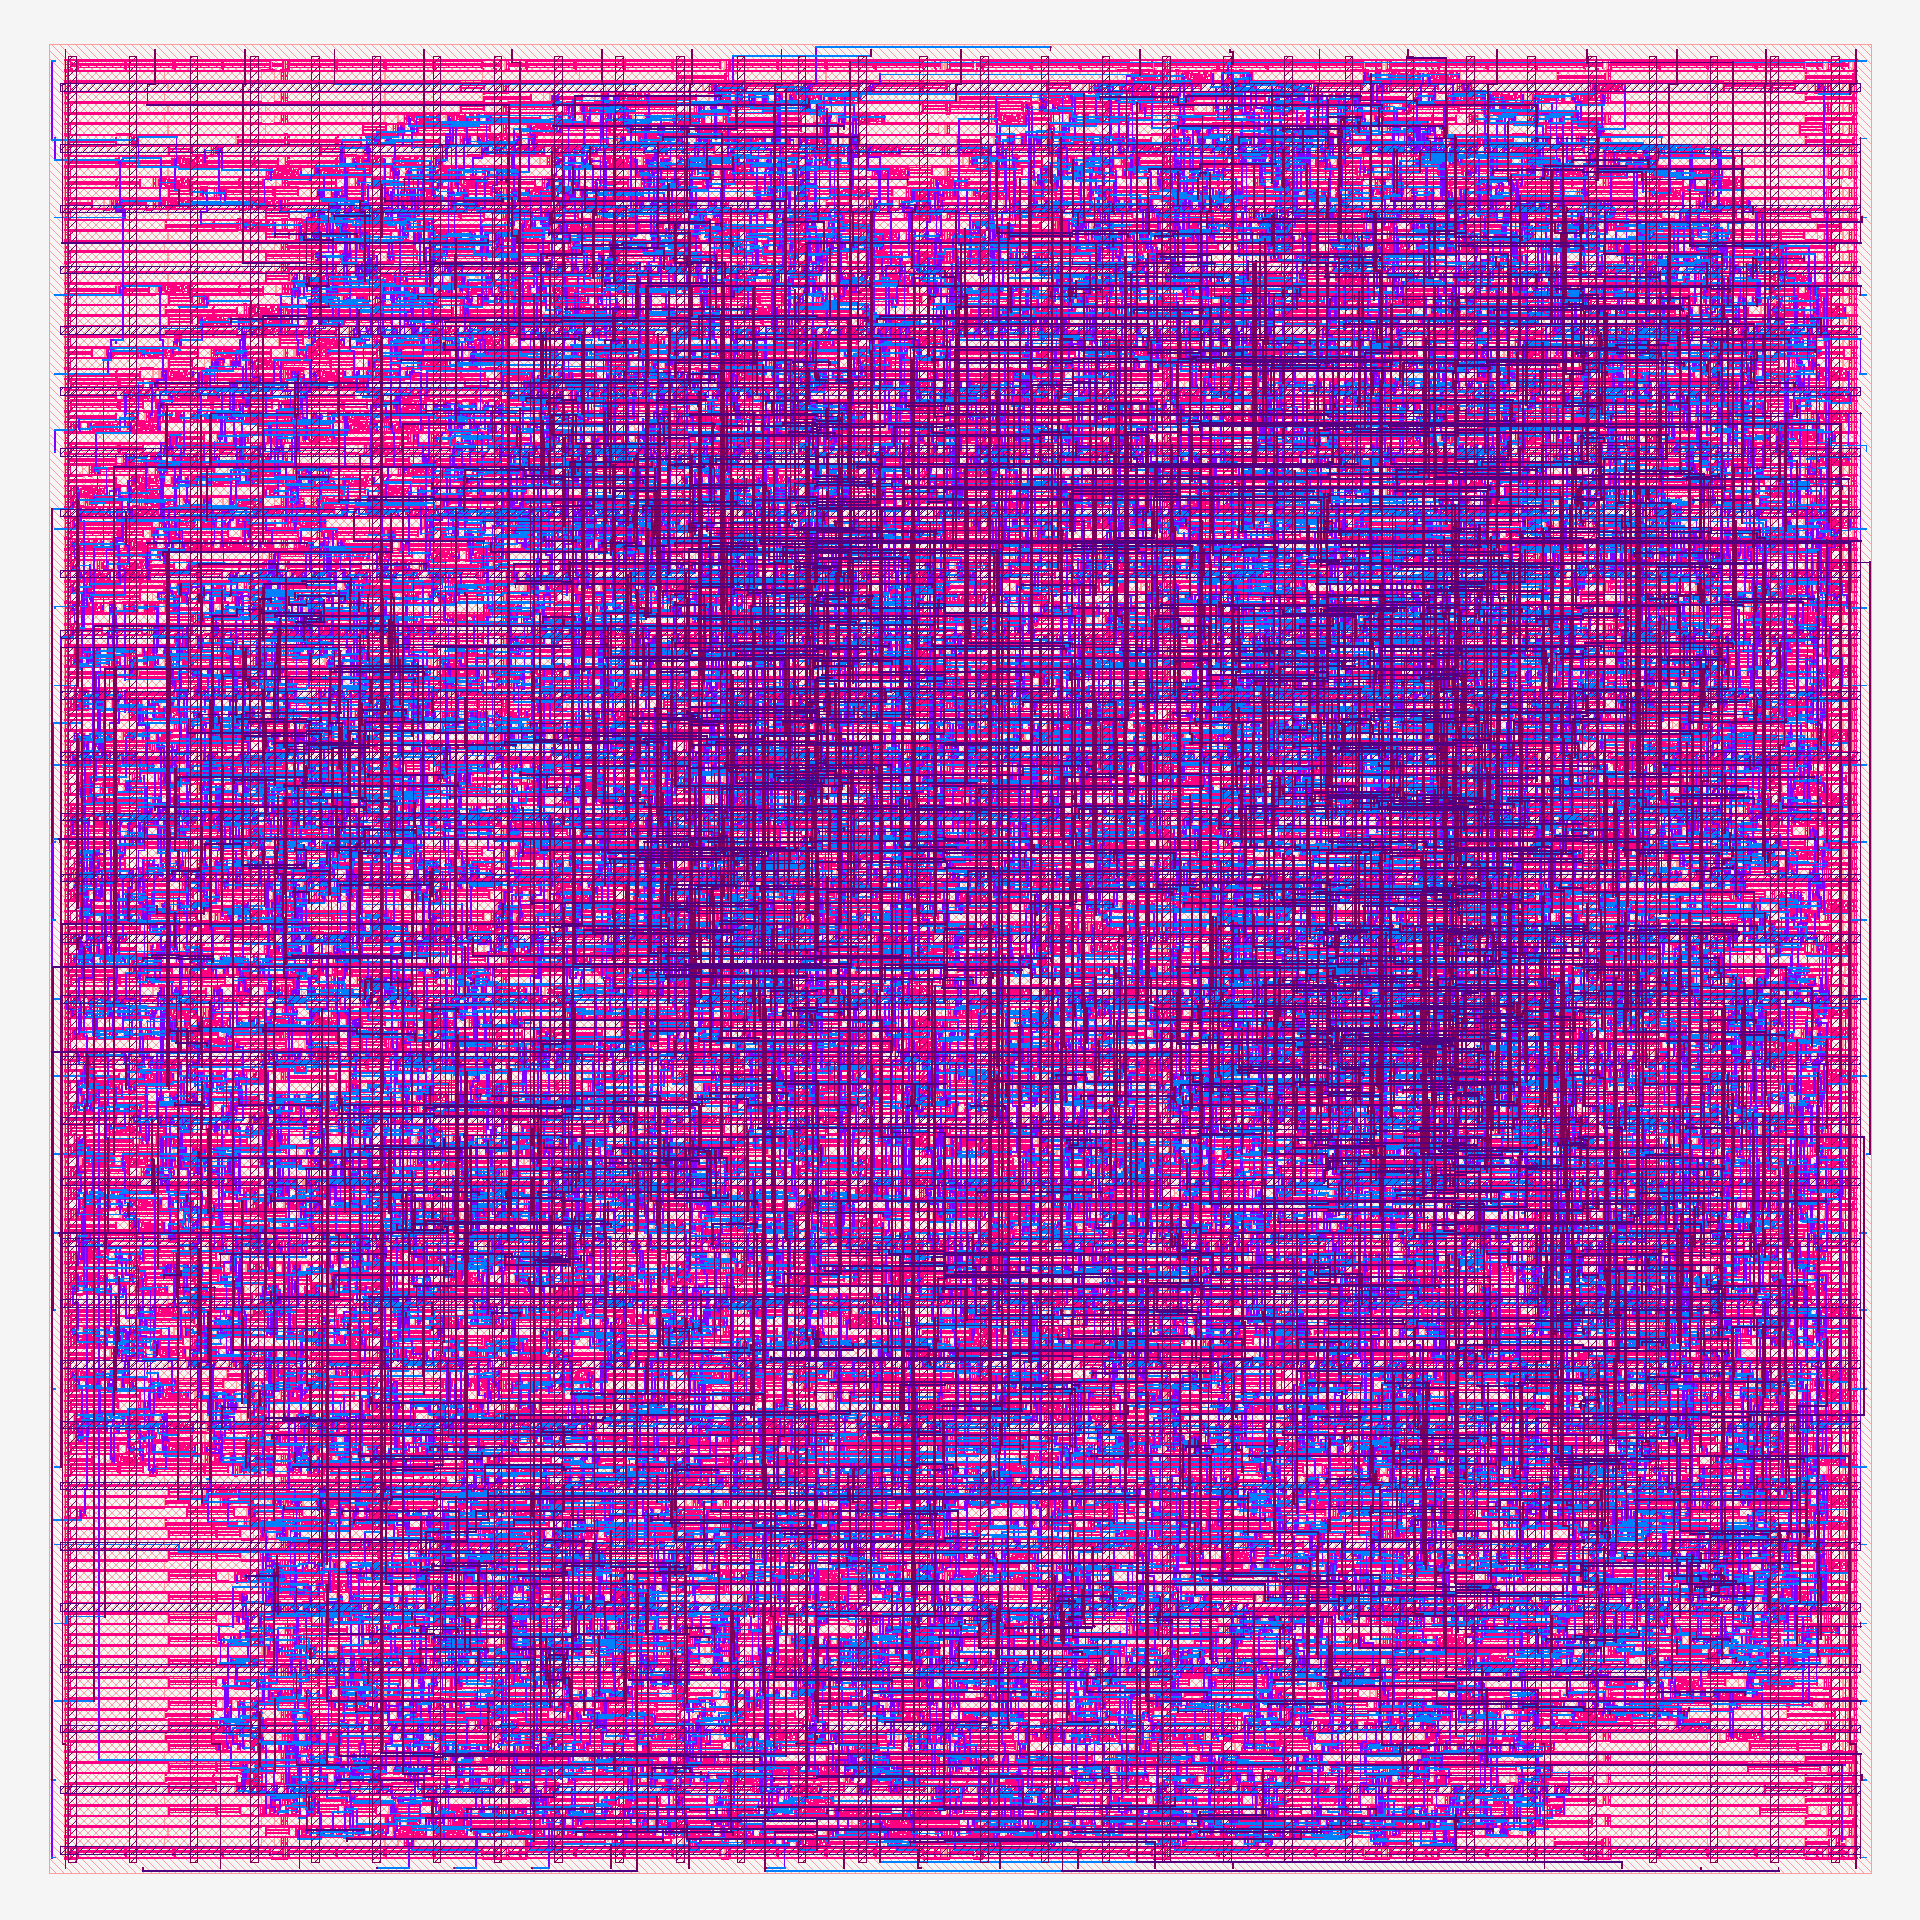
\includegraphics[width=0.88\linewidth,height=0.70\textheight,keepaspectratio]{xinghuo-npu-tile.png}
\caption{“星火”NPU Tile 版图视图（ECOS Studio 后端导出）。}\label{fig:layout}
\end{figure}
\end{document}
